\documentclass{beamer}

\usepackage{amsmath, amssymb}
\usepackage[utf8]{inputenc}
\usepackage{macros}
\usepackage{minted}
\usemintedstyle{trac}
\usepackage[T1]{fontenc}
\usepackage{lmodern} 
\usefonttheme{serif}



% \usepackage{pgfpages}
% \pgfpagesuselayout{resize to}[a4paper,border shrink=5mm,landscape]

% \usefonttheme{professionalfonts}
\setbeamertemplate{navigation symbols}{}

\definecolor{Black}{rgb}{0,0,0}


% Make 
\setbeamertemplate{frametitle}{
    \color{black}
    \insertframetitle{}
    \par
    \vskip-6pt
    \hrulefill}
    
    % Set slide title color
    \setbeamercolor{title}{fg=Black} 
    
    \setbeamertemplate{itemize items}[default]
    \setbeamertemplate{enumerate items}[default]
    
    \setbeamertemplate{itemize items}[circle]
    \setbeamercolor{itemize item}{fg=Black}
    \setbeamercolor{itemize subitem}{fg=Black}
    \setbeamercolor{itemize subsubitem}{fg=Black}
    
    
    \setbeamercolor{enumerate item}{fg=Black}
    \setbeamercolor{enumerate subitem}{fg=Black}
    \setbeamercolor{enumerate subsubitem}{fg=Black}
    
    
    % --- page number ---
    \setbeamertemplate{footline}{%
	\raisebox{10pt}{\makebox[\paperwidth]{\hfill\makebox[7em]{\normalsize\texttt{\insertframenumber/\inserttotalframenumber}}}}%
    }
    
    % Presenter's note
% \setbeameroption{show notes on second screen}

\title{Presentation title}
\author{Mateusz Kojro}
\date{\today}

\begin{document}

    \begin{frame}[plain]
        \maketitle
    \end{frame}

    
    \begin{frame}{Slide title}
        Innner text
        \note{
            Please write presenter's note here.
        }
    \end{frame}

    \begin{frame}[fragile]{Some source code}
            \begin{minted}[frame=single,linenos]{cpp}
#include <iostream>
int main() { // Thats a main function
    std::cout << "Hello world!" << std::endl;    
    return 0;
}
            \end{minted}
    \end{frame}

    \begin{frame}[plain,c]
        \begin{center}
            \Large Setcion title
        \end{center}
    \end{frame}

    \begin{frame}{Some highlighting}

        \begin{itemize}

            \item{\highlight{ \text{Simple highlight}}}
            \item{\highlight[blue]{ \text{Other color}}}
            \item{$\highlightcapoverlay{\sum{x}}{Caption can be overlayed}$}
            \item{$\highlightcap[blue]{\int_a^b e^x dx}{or not move the equation to the right place}$}

            \begin{enumerate}
                \item{one}
                \item{two}
            \end{enumerate}
        \end{itemize}

    \end{frame}

    \begin{frame}{Lets do some graphs}
        \begin{columns}[c]
            \begin{column}{0.6\hsize}\centering
                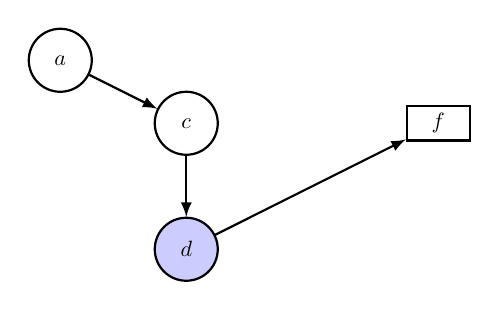
\begin{tikzpicture}[thick,scale=0.8, every node/.style={scale=0.8}]
                    \node[draw, circle, minimum width=1cm] (a) at (-2, 1) {$a$};
                    \node[draw, circle, minimum width=1cm] (c) at (0, 0) {$c$};
                    \node[draw, rectangle, minimum width=1cm] (f) at (4, 0) {$f$};
                    \node[draw, circle, minimum width=1cm, fill=blue!20!white] (d) at (0, -2) {$d$};
                    
                    \draw[-latex] (a) -- (c);
                    \draw[-latex] (c) -- (d);
                    \draw[-latex] (d) -- (f);
                \end{tikzpicture}
            \end{column}
            \begin{column}{0.4\hsize}
                \begin{itemize}
                    \item Item 1
                    \item Item 2
                    \item Item 3
                \end{itemize}
            \end{column}
        \end{columns}
    \end{frame}
\end{document}
